\subsection{OB-6 (APS)}
\label{OB-6}
HW podpora virtualizace hlavní paměti stránkováním, funkce MMU (Memory Management Unit) a překlad virtuálních adres na fyzické adres pomocí TLB (Translation Lookaside Buffer), ošetření výpadku stránky.

\textbf{Problémy bez virtualizace (motivace pro virtuální paměť):}
\begin{itemize}
	\item Velikost paměti: paměť nemusí být dost velká pro spuštění procesu.
	\item Fragmetace: Při ukončování procesů vzniknou v hlavní paměti volá místa různých velikostí.
	\item Dynamická alokace: Jak alokovat další paměť?
	\item Bezpečnost: Jak zařídit, aby si procesy nemohly číst paměť navzájem?
\end{itemize}

\textbf{Jak funguje stránkování?}
\begin{itemize}
	\item uživatelským procesům je nabídnut Virtuální Adresní Prostor (VAP)
	\item každý proces má svůj VAP
	\item VAP je rozdělen na stejně velké \textit{stránky}, hlavní paměť (HP) je rozdělena nastejně velké \textit{rámce}.
	\item běžící procesy do rámců HP umisťují momentálně potřebné stránky svého VAP (pracovní množina)
	\item nepoužívané stránky se při nedostatku paměti odloží na disk
	\item mapování VAP do HP a přenos stránek mezi HP a diskem zajišťuje OS
	\item virtuální adresa se skládá z čísla stránky a offsetu
	\item fyzická adresa se skládá z čísla rámce a offsetu
\end{itemize}

\textbf{Možnosti překladu virtuálních adres na fyzické:}
\begin{itemize}
	\item Konvenční stránkovací tabulka
	
	Každý proces má svou stránkovací tabulku (většinou strom stránkovacích tabulek).	
	
	\item Inverzní stránkovací tabulka
	
	Všechny procesy sdílejí jedinou, inverzní stránkovací tabulku.
\end{itemize}

\textbf{Jednoúrovňová stránkovací tabulka:}
\begin{itemize}
	\item pro překlad se použije číslo stránky jako index do tabulky, a tam se najde číslo rámce
	\item jednoúrovňová tabulka je ale i pro 32bitové systémy velká, a když ji má každý proces, zabere to hodně místa
\end{itemize}

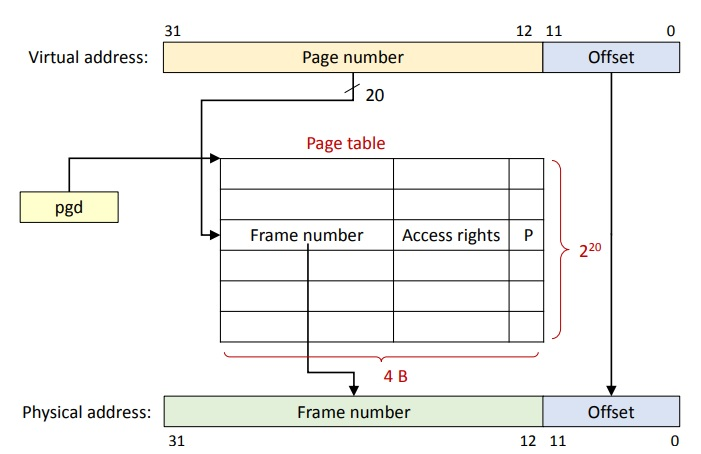
\includegraphics[width=0.8\textwidth]{img/OB-6_0.jpg}

\newpage
\textbf{Víceúrovňové stránkovací tabulky:}
\begin{itemize}
	\item pro překlad se použije číslo stránky, které je složené z indexů do různých úrovní stránkovacích tabulek
	\item jednotlivé tabulky jsou zásadně menší, na počátku stačí jedna tabulka v každé úrovni, další OS může podle potřeby přidat
\end{itemize}

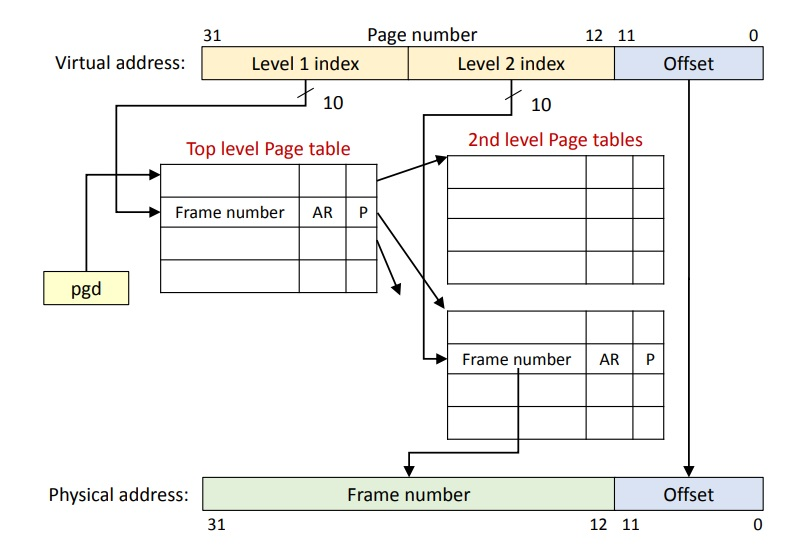
\includegraphics[width=0.8\textwidth]{img/OB-6_1.jpg}

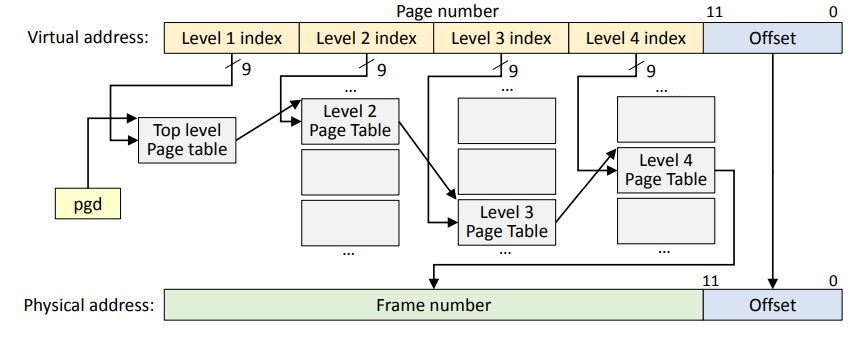
\includegraphics[width=0.8\textwidth]{img/OB-6_2.jpg}

Při překladu VA na FA se musí procházet několik úrovní tabulek stránek (page walk). Ty mohou být uloženy mimo paměť a může dojít k výpadku stránky (page fault).

\subsubsection*{MMU --- Memory Management Unit}
\begin{itemize}
	\item vykonává page walk
	\item dostane adresu stránkovací tabulky první úrovně přes domluvený registr
	\item pokud nedokáže přeložit adresu, nastává page fault, a procesor generuje výjimku
	\begin{itemize}
		\item Invalid page fault --- adresa není součístí adresního prostoru procesu --- obvykle porces zastaven se segmentation fault
		\item Valid page fault --- adresa je součástí VAP, ale nezle přeložit (nenachází se v MMU, tedy musí page walk vykonat OS / překlad neexistuje --- stránka není v HP ale na disku --- OS vymění stránky v HP)
	\end{itemize}
\end{itemize}

\subsubsection*{TLB --- Translation Lookaside Buffer}
Vykonávání page walk je časově náročný proces. Aby nebylo nutné pokaždé page walk vykonávat, každá MMU používá speciální HW překladovou tabulku --- TLB.

TLB jako přímo mapovaná cache:

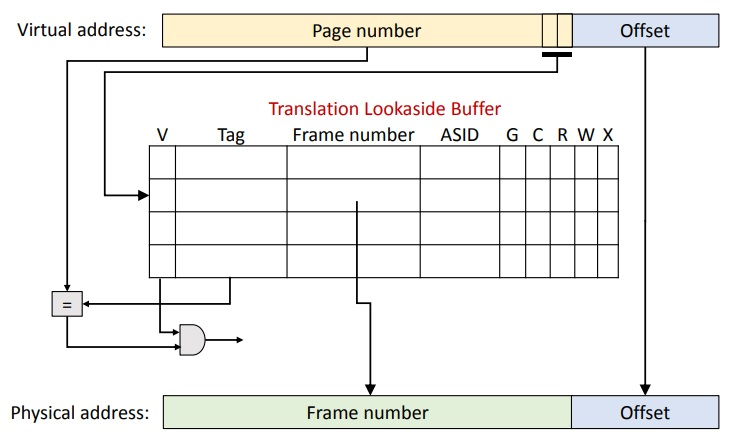
\includegraphics[width=0.8\textwidth]{img/OB-6_3.jpg}

Typicky se používá stupeň asociativity 4-64. Podobně jako u cache se používá SRAM.

Každá položka TLB typicky obsahuje:
\begin{itemize}
	\item V: validity bit
	\item Tag: číslo stránky (část)
	\item Frame number: číslo rámce
	\item ASID: Identifikátor adresního prostoru (pro oddělení procesů)
	\item G: global flag (pokud G = 1, ASID se ignoruje)
	\item C: cache policy (informace, jestli jsou data na adrese "cachovatelná" --- pro I/O zařízení, kam se změny dat musí posílat rovnou)
	\item Access permissions: R, W, X
\end{itemize}

\textbf{Sumarizace HW podpory:}

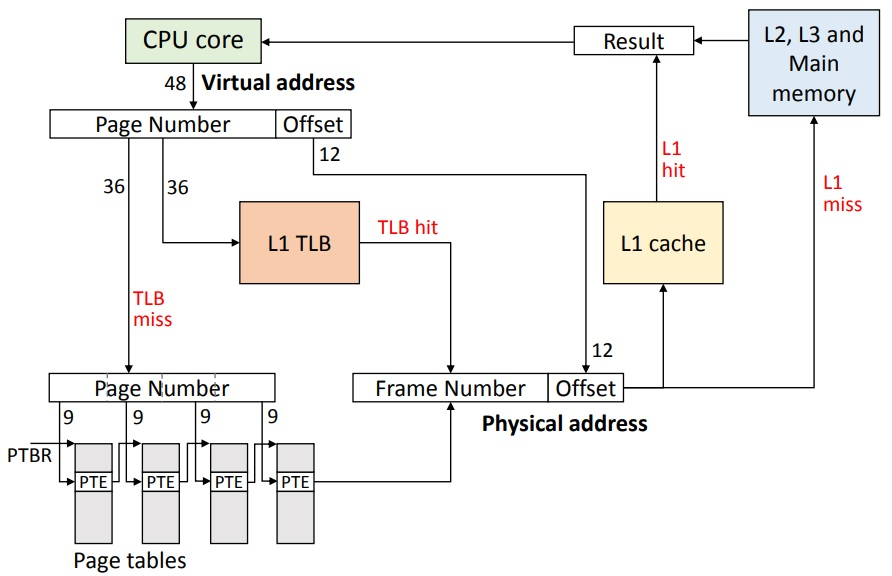
\includegraphics[width=0.8\textwidth]{img/OB-6_4.jpg}